\documentclass[a4paper,10pt]{article}
\usepackage[T1]{fontenc}
\usepackage[utf8]{inputenc}
\usepackage[english]{babel}
\usepackage{lmodern}
\usepackage[top=1.6cm,bottom=1.8cm,left=1.9cm,right=1.9cm]{geometry}
\usepackage{titlesec,enumitem,xcolor,graphicx,lastpage,fancyhdr}
\usepackage{fontawesome5}
\usepackage[hidelinks]{hyperref}

\hypersetup{colorlinks=true,urlcolor=blue!70!black,linkcolor=blue!70!black}
\pagestyle{fancy}\fancyhf{}\renewcommand{\headrulewidth}{0pt}
\fancyfoot[C]{\small\color{gray}Page \thepage\ of \pageref{LastPage}}
\setlength{\parindent}{0pt}

\titleformat{\section}{\large\bfseries\color{blue!70!black}}{}{0em}{}[\vspace{-0.7em}\rule{\textwidth}{0.5pt}]
\titlespacing{\section}{0pt}{9pt}{5pt}
\setlist[itemize]{leftmargin=1.1em,itemsep=2pt,topsep=2pt,parsep=0pt}
\newcommand{\role}[4]{\vspace{3pt}\noindent\hspace{0.6em}\parbox[t]{0.38\textwidth}{\raggedright\textbf{#1}}\hfill\parbox[t]{0.58\textwidth}{\raggedleft\textit{#2}}\\{\textit{#3}\hfill\textit{#4}}\vspace{1pt}}

\begin{document}
\noindent
\begin{minipage}[t]{0.78\textwidth}
\vspace{0pt}
{\huge\bfseries Prabhavit Gupta}\\[8pt]
{\small \faPhone\ +39-351-610-7807 \quad \faEnvelope\ \href{mailto:prabhavitg@gmail.com}{prabhavitg@gmail.com} \quad \faLinkedin\ \href{https://www.linkedin.com/in/prabhavit/}{Linkedin} \quad \faMapMarker*\ Venice, Italy}
\end{minipage}\hfill
\begin{minipage}[t]{0.18\textwidth}
\vspace{0pt}\raggedleft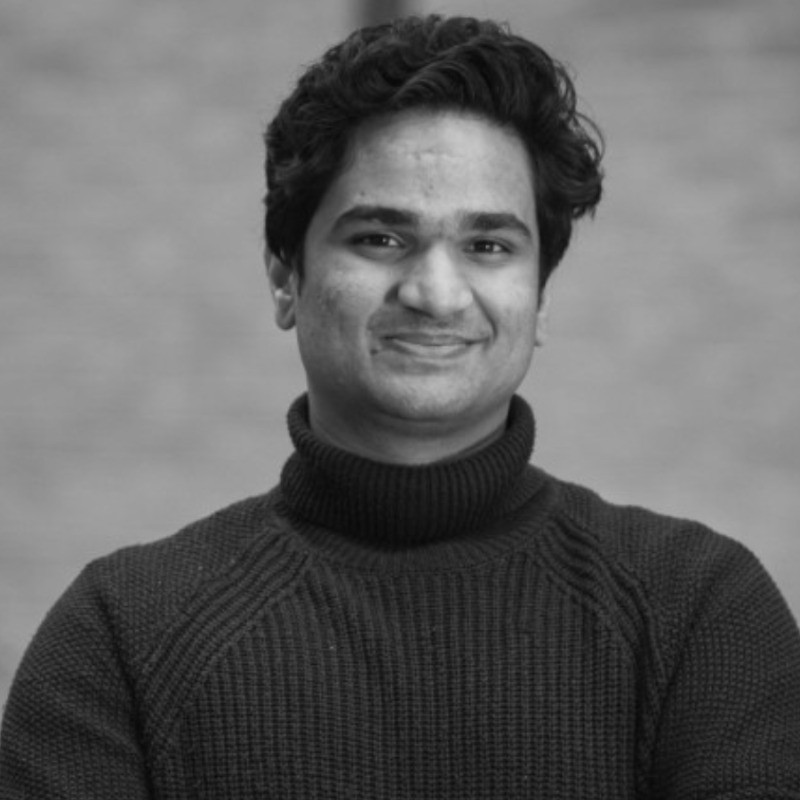
\includegraphics[width=2.3cm,height=2.3cm,keepaspectratio]{photo.jpg}
\end{minipage}

\section{Career Summary}
\begin{itemize}
\item Automation Project Engineer with dual degrees in Mechanical Engineering and Management Engineering (Politecnico di Milano), experienced in industrial automation project lifecycle and systems integration.
\item Solid foundation in pharmaceutical automation engineering, computerized systems qualification (URS, FDS, FAT/SAT, CSV/GAMP), and standard operating procedure (SOP) drafting.
\item Hands-on background with PLC/SCADA systems, continuous historian databases, OT network segregation, and industrial change control protocols.
\item Experienced in project budgeting, vendor contract coordination, cross-functional stakeholder alignment (QA, Production, Maintenance), and technology innovation scouting.
\end{itemize}

\section{Technical Skills}
\begin{itemize}
\item \textbf{Automation \& Control Systems} -- PLC Programming Logic (Siemens, Rockwell), SCADA Systems, BMS, DCS Fundamentals, Traceability Vision Systems
\item \textbf{Pharma Project \& Quality} -- User Requirements Specifications (URS), GAMP 5, GMP Compliance, Computerized Systems Validation (CSV), Change Control, SOPs
\item \textbf{OT Infrastructure \& Cybersecurity} -- OT Network Segregation, Industrial Ethernet, Profinet, Modbus, NIS2 Cybersecurity Awareness, Historian Databases
\item \textbf{Project Management \& Engineering} -- Feasibility Studies, Budget \& Cost Tracking, Vendor Procurement \& Subcontractor Management, Site Commissioning (Collaudo)
\item \textbf{Software \& Tools} -- Python, SQL, Relational Databases, Linux, Git, Jira, Technical Documentation
\end{itemize}

\section{Visa \& Language}
\begin{itemize}
\item \textbf{Language} -- Italian (Conversational / Intermediate), English (Fluent / Professional), Hindi (Native)
\item \textbf{Work Authorization} -- European Long Term Residence Permit (No Visa Sponsorship required). Driving License (Patente B). Available for on-site travel to Parma.
\end{itemize}

\section{Professional Experience}
\role{\href{https://flowspace.co}{FlowSpace.co}}{Automation Project \& Systems Lead}{London, UK / Remote}{Mar 2024 -- Ongoing}
\begin{itemize}
\item \textbf{Project Management \& Technical Delivery:}
\begin{itemize}[label=--]
\item Managed end-to-end delivery of automated process systems and data pipelines, aligning technical specifications with stakeholder operational goals.
\item Formulated detailed requirement specifications (URS), technical work scopes, and acceptance testing protocols for external suppliers.
\item Tracked project milestones, resource allocation, and budget variance, delivering complex milestones on schedule.
\end{itemize}
\item \textbf{Systems Validation \& Continuous Quality:}
\begin{itemize}[label=--]
\item Authored validation documentation, technical SOPs, and system change control procedures maintaining stringent compliance standards.
\item Supervised continuous platform upgrades and telemetry integrations, sustaining 99.9\% operational availability across production services.
\end{itemize}
\item \textit{Tools: Python, Linux, Relational Databases, SQL, REST APIs, Git, Project Management}
\end{itemize}

\role{Urlink}{Systems Automation Engineer}{Milan, Italy}{Jul 2023 -- Feb 2024}
\begin{itemize}
\item Supported site engineering teams in commissioning, qualification, and acceptance testing (collaudo) of automated production equipment.
\item Liaised with cross-functional quality and operations departments to verify automated data acquisition and sensor telemetry against specifications.
\item Drafted commissioning checklists, hardware interface protocols, and maintenance SOPs for manufacturing technicians.
\end{itemize}

\role{UltraStrategy}{Automation Developer}{Remote, Germany}{Sep 2022 -- Jun 2023}
\begin{itemize}
\item Developed Python automation routines tracking equipment cycle parameters and efficiency metrics across industrial operations.
\item Generated structured reporting pipelines summarizing machine uptime, process trends, and quality compliance metrics.
\end{itemize}

\section{Education}
\role{Politecnico di Milano}{M.Sc. in Management Engineering (Digital Business \& ICT)}{Milan, Italy}{2020 -- 2023}
\role{Thapar Institute of Engineering and Technology}{B.E. in Mechanical Engineering}{Punjab, India}{2014 -- 2018}

\end{document}
